\documentclass{article}
\usepackage[utf8]{inputenc}
\usepackage{kpfonts}
\usepackage{commath}
\usepackage{amsthm}
\usepackage{graphicx}
\usepackage[margin=0.8in]{geometry}

\newcommand{\R}{\ensuremath{\mathbb{R}}}
\newcommand{\N}{\ensuremath{\mathbb{N}}}
\newcommand{\Q}{\ensuremath{\mathbb{Q}}}
\newcommand{\B}{\ensuremath{\mathcal{B}}}
\newcommand{\card}[1]{\ensuremath{\mathbf{card} (#1)}}
\newcommand{\func}[1]{\ensuremath{#1:\R \to \R}}
\newcommand{\Iff}{if and only if}
\newcommand{\nbd}{neighborhood}
\newcommand{\closure}[1]{\ensuremath{\overline{#1}}}
\newcommand{\ball}[3][\empty]{\ensuremath{B^{#1}_{#2}(#3)}}
\newcommand{\Ball}[3][\empty]{\ensuremath{\overline{B}^{#1}_{#2}(#3)}}
\newcommand{\fRR}{\ensuremath{f:\R \to \R}}
\newcommand{\define}[1]{\textbf{\underline{#1}}}
\newcommand{\ts}{topological space}
\newcommand{\tp}{\ensuremath{\mathcal{T}}}
\newcommand{\Ts}[2]{\ensuremath{(#1,#2)}}
\newcommand{\es}{\ensuremath{\emptyset}}
\newcommand{\tpcof}{\ensuremath{\tp_\text{cof}}}
\newcommand{\tpdisc}{\ensuremath{\tp_\text{disc}}}
\newcommand{\tptriv}{\ensuremath{\tp_\text{triv}}}
\newcommand{\union}{\cup}
\newcommand{\Union}{\bigcup}
\newcommand{\inter}{\cap}
\newcommand{\Inter}{\bigcap}
\newcommand{\interior}[1]{\ensuremath{\mathring{#1}}}
\newcommand{\bound}[1]{\ensuremath{\partial #1}}
\renewcommand{\Subset}{\subseteq}
\renewcommand{\Supset}{\supseteq}

\theoremstyle{definition}
\newtheorem*{defn}{Definition}
\newtheorem*{thm}{Theorem}
\newtheorem*{prop}{Proposition}
\newtheorem*{ex}{Ex}

\theoremstyle{remark}
\newtheorem*{rem}{Remark}

\begin{document}
    \begin{center}
        \textsc{Dillan Marroquin\\MATH 440.1001\\Scribing Week 4\\Due. 22 February 2021\\}
    \end{center}
    
    \subsection*{Review of Last Lecture}
        \begin{thm}[9.5]
            Let $A \Subset X$ be a subset of a \ts{} $X$. Then $\closure{A} = A \union L(A)$.
        \end{thm}
        
    \noindent\section*{\textbf{\textsc{Lecture 10}}}
        \begin{prop}[10.1]
            Let $X$ be a space, $Y \Subset X$ a subspace. Then $B \Subset Y$ is closed in $Y$ \Iff{} there exists a closed subset $A \Subset X$ such that $B = Y \inter A$. 
        \end{prop}
        
        \begin{proof}[10.1]
        ($\implies$) Suppose $B \Subset Y$ is closed. Recall that the subspace topology on $Y$, $W \Subset Y$, is open \Iff{} $W=Y \inter U$ for some open $U \Subset X$:
        \begin{center}
            \graphicspath{images}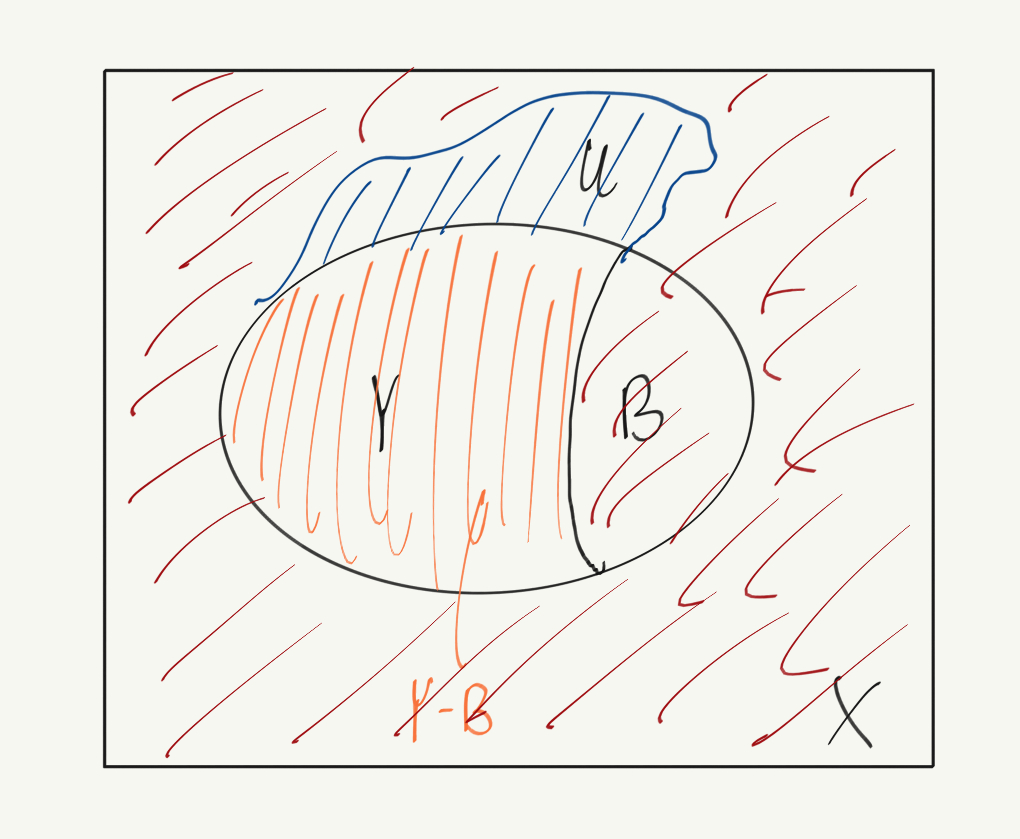
\includegraphics[scale = 0.15]{images/Proof 10.1.png}
        \end{center}
        ($\impliedby$) Suppose $B = Y \inter A$, $A \inter X$ closed. We want to show $B$ is closed in $Y$, that is, $Y-B$ is open in $Y$. To do this, we work backwards from the picture above.
        \end{proof}
    \subsection*{Closure is a Relative Notion\ldots}
        \begin{ex}[10.2] Find $\closure{A}$.
            \begin{enumerate}
                \item Let $A = [-1,0) \Subset \R$. What is $\closure{A}$?\\
                \indent$\closure{A} = A \inter L(A) = [-1,0]$ as a subset of $\R$.
                
                \item Let $Y=[-1,0] \union (0,2] \Subset \R$. Give $Y$ the subspace topology. Now $A=[-1,0) \Subset Y$. What is $\closure{A}$?\\
                \indent Note: $A=Y \inter [-1,0]$. Prop 10.1 implies $A$ is a closed subset of $Y$ which implies $\closure{A} = A$ as a subset of $Y$.
            \end{enumerate}
        \end{ex}
        
        \begin{defn}[10.3]
            Let $X$ be a space, $A \Subset X$. The \define{interior} of $A$, \define{$\interior{A} = \mathrm{Int}(A)$}, is the union of all open subsets contained in $A$.\\
            The \define{boundary} of $A$ is the subset \define{$\bound A := \closure{A} - \interior{A}$}.
        \end{defn}
        
        \begin{rem}[10.4] Facts about $\interior{A}$ and $\bound A$.
            \begin{enumerate}
                \item $\interior{A}$ is open in $X$ and is the "largest" open subset of $X$ contained in $A$.
                \item $\bound A \Subset X$ is a closed subset of $X$: $\bound A = \closure{A} \inter (X-\interior{A})$.
            \end{enumerate}
        \end{rem}
        
        \begin{ex}[10.5] A few examples involving $\interior{A}$ and $\bound A$.
            \begin{enumerate}
                \item $X = \R, \, A=(0,1)$.\\
                \indent $\interior{A} = A, \, \closure{A} = [0,1],\, \bound A = \closure{A} - \interior{A} = \{0,1\}$.
                \item $X = \R^2, \, A=\Ball{x}{\varepsilon}$.\\
                \begin{center}
                    \graphicspath{images}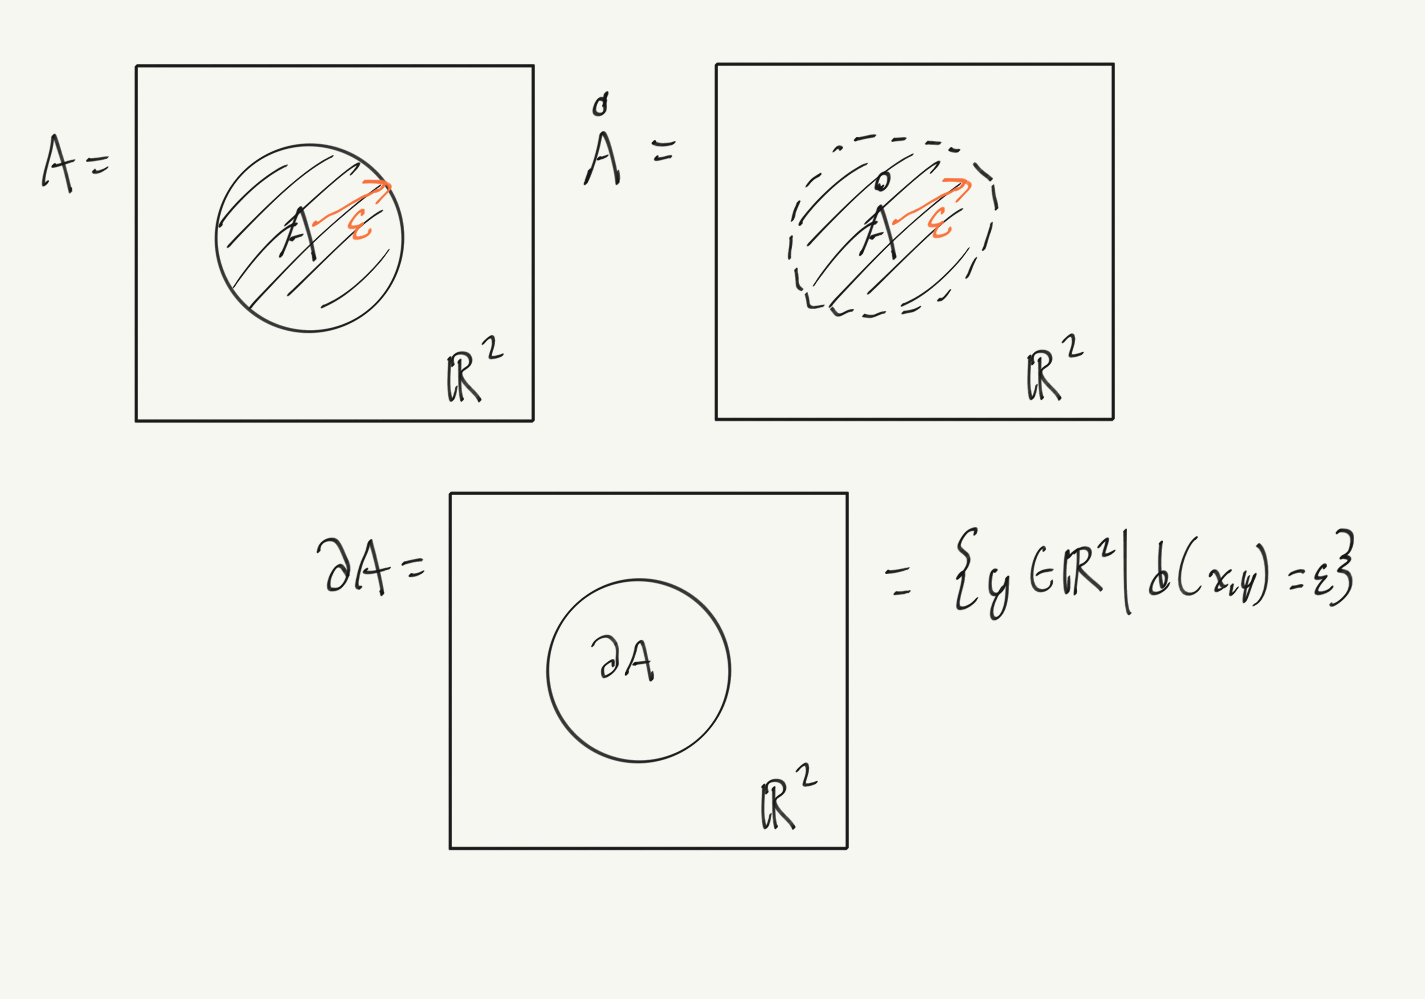
\includegraphics[scale = 0.15]{images/Ex 10.5.png}
                \end{center}
            \end{enumerate}
        \end{ex}
        
        \begin{prop}[10.6]
            Let $X$ be a space. Let $A \Subset X, \, x \in X$. Then $x \in \interior{A}$ \Iff{} there is an open \nbd{} $V \Subset X$ of $x$ such that $V \Subset A$.
        \end{prop}
        
        \begin{prop}[10.7]
            Let $X$ be a space, $A \Subset X, \, x \in X$. Then $x \in \bound A$ \Iff{} for every open \nbd{} $U \Subset X$ of $x$, we have $U \inter A \neq \emptyset$ and $U \inter (X-A) \neq \emptyset$.
        \end{prop}
    \section*{\textbf{\textsc{Lecture 11}}}
        \subsection*{Important Use of Closure}
            \begin{itemize}
                \item Recall from Real Analysis: $\forall x \in \R$ and $\forall \varepsilon > 0, \, \exists q \in \Q$ such that $r-\varepsilon < q < r+\varepsilon$.
                \item Important consequence of this: Every continuous function $\func{f}$ is uniquely determined by its value on rationals, i.e. if $\func{f,g}$ are continuous and $\forall q \in \Q$ where $f(q)=g(q)$, then $f=g$.
            \end{itemize}
            \begin{defn}[11.1]
                Let $X$ be a \ts. A subset $A \Subset X$ is \define{dense} \Iff{} $\define{\closure{A} = X}$.\\
                We say $X$ is \define{separable} \Iff{} $X$ contains a countable dense subset, i.e. $\exists A \Subset X$ such that $\card{A} = \card{\N}$ and $\closure{A} = X$.
            \end{defn}
        
        \subsection*{Main Examples}
            \begin{itemize}
                \item $\Q \Subset \R$ is dense and countable in Euclidean space.
                \item $\Q^n \Subset \R^n$ is dense and countable. Therefore $\Ts{\R^n}{\tp_{\text{Euclid}}}$ is separable.
                \item $\Ts{\R}{\tpcof}$. Let $U \Subset \R$ be open and non-empty. By definition of $\tpcof$, $\R-U$ is a finite subset of $\R$.\\
                $\closure{U} = \R \implies U$ is dense in $\R$.
            \end{itemize}
            
        \subsection*{Section M13: Basis for Topologies}
            \begin{itemize}
                \item In this section, we will generalize open balls in Euclidean space.
                \item Recall how we characterized open subsets of $\R^n$: $U \Subset \R^n$ is open \Iff{} $U = $ union of open balls.
            \end{itemize}
        
            \begin{defn}[11.2]
                If $X$ is a set, a \define{basis for a topology} on $X$ is a collection $\B$ of subsets of $X$ such that
                \begin{enumerate}
                    \item For each $x \in X$, there is at least 1 basis element $B \in \B$ such that $x \in B$.
                    \item If $B_1,B_2 \in \B$ and $x \in B_1 \inter B_2$, then there exists a $B_3 \in \B$ such that $x \in B_3 \Subset B_1 \inter B_2$:
                    \begin{center}
                        \graphicspath{images}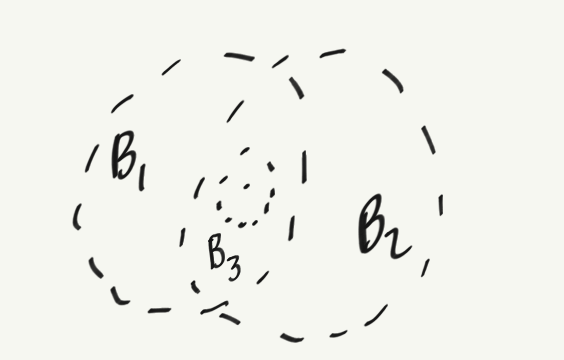
\includegraphics[scale = 0.2]{images/Basis for a Topology.png}
                    \end{center}
                \end{enumerate}
            \end{defn}
            
            Key Idea: If $\B$ is a basis for a topology on a set $X$, then the topology generated by $\B$, $\tp_\B$, is as follows:
            \begin{align*}
                U \in \tp_\B \text{ is open \Iff{} } \forall x \in U, \, \exists B \in \B \text{ such that } x \in B \text{ and } B \Subset U.\, \Ts{X}{\tp_\B}
            \end{align*}

            \begin{prop}[11.3]
                $A \Subset X$ is dense \Iff{} $A \inter U \neq \emptyset$ when $U$ is any non-empty open subset of $X$.
            \end{prop}
\end{document}